% 事件与尺缩效应
% 事件|狭义相对论|时空坐标|同时性|相对性|火车佯谬|尺缩效应

\pentry{狭义相对论的基本假设\upref{SpeRel}}

\subsection{事件}

在和时空相关的理论中,当我们描述一件事的时候,我们并不关心这件事具体是什么,只关心它发生在何时何地.因此为了将来的讨论,我们首先需要定义“事件”的概念.

一个\textbf{事件(event)}是指在时空坐标系中的一个点.事件所发生的时间、地点,就是事件作为一个点的坐标.

\subsection{对事件的观测}

狭义相对论的核心是光.在任何参考系中,光速不变.光的其它性质并不能保证一定不变,如光强的分布,偏振的角度等.

除了光速以外,事件本身也是不随惯性系变化的.这就是说,在任何惯性系$K_1$中同时同地发生的事情,在任何惯性系$K_2$中也是同时同地发生的.鉴于我们已经为了简便,将事件简单表达为它所发生的时间和地点,那么同时同地发生的事件都应看成同一个事件.

更进一步,由于讨论事件时我们只关心其发生的时间和位置,即只关心其时空坐标,因此也可以直接用\textbf{事件的时空坐标}来指代\textbf{事件本身}.

光速和事件的不变性,是目前我们观测事件的最基本工具.我们将在实践中体会利用光速不变和事件不变来观测事件的方法.

\subsection{同时性的相对性}

考虑一根的铁轨,向左向右都无限延伸.在这铁轨上取一个点作为原点,向右作为正方向,可以画一个$x_1$轴,用来测量和铁轨静止的参考系中的事件位置,这个参考系称作\textbf{铁轨系},记为$K_1$.

现在,铁轨上从左到右开过一辆火车.和火车静止的参考系也可以沿着铁轨画一个$x_2$轴,只不过它是用来描述火车参考系中事件位置的,称作\textbf{火车系},记为$K_2$.

在铁轨系中,如果某时刻看到火车的两个不重叠的轮子同时发光,那么这两道光会在铁轨上的两个发光点的中点相遇,而“相遇”也是一个事件.从发光到相遇,两束光通过了相同的路程,由于光速不变,它们经过了相同的时间,由此反推可知发光的时间是一样的.但是同样的三个事件在火车系看来是不一样的:在火车系中,“相遇”发生在更靠近后轮的位置,也就是说,在火车看来前轮所发的光走过了更长的路程,花了更长的时间,从“相遇”的时间反推回去,可知在火车眼里是前轮先发光.

\begin{figure}[ht]
\centering
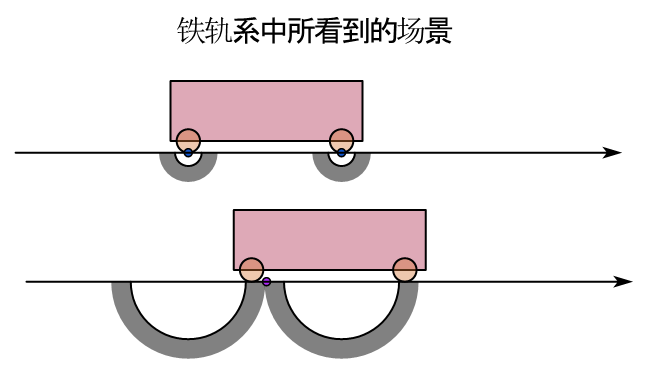
\includegraphics[width=8cm]{./figures/SRsmt_1.png}
\caption{在铁路系中所看到的三个事件,分别用三个点表示.上图是两个轮子同时发光的两个事件;下图是一段时间以后,火车运动了一段距离,而两束光相遇的事件.} \label{SRsmt_fig1}
\end{figure}

事实上,在$K_1$中同时但不同地发生的事情,在$K_2$中必然不同时发生.“同时”这一概念并非绝对,两个事件是否同时,取决于从什么参考系来观察它们.

\begin{exercise}{火车系中的事件}

\autoref{SRsmt_fig1} 中是以铁轨的视角,选取了两个时刻,描述了“前轮发光”、“后轮发光”和“光束相遇”这三个事件.请你尝试画出火车的视角下三个事件的先后关系.提示:你需要三个关键时刻,依次是“前轮发光”时,“后轮发光”时和“光束相遇”时.

\end{exercise}

\subsection{尺缩效应}

我们还是使用上一节定义的火车系$K_2$和铁轨系$K_1$.如果说,在铁轨上标记了两个点$A$和$B$,使得前轮通过$B$时发光,后轮通过$A$时发光.在$K_1$中,前轮和后轮分别同时通过这两个点,也就是说,在$K_1$中,火车两轮的间距和$A$、$B$的间距一样;但是在$K_2$中来看,前轮先发光,后轮后发光,这就意味着火车两轮的间距比$A$、$B$的间距要长.

这说明,运动的物体应该比静止时看起来要短.由于没有任何点是特殊的,所以这种运动造成的收缩在每一个地方都是一样的,或者说,运动造成的尺缩效应是均匀的.那么运动造成的收缩的比例应该怎么计算呢?

\begin{figure}[ht]
\centering
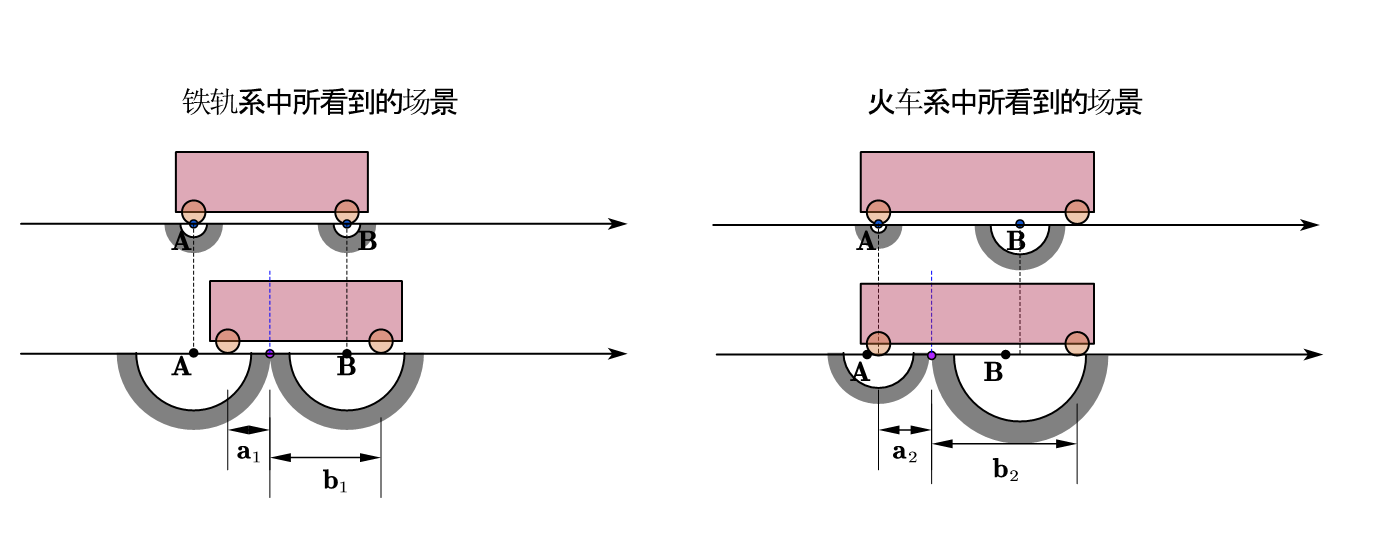
\includegraphics[width=14.5cm]{./figures/SRsmt_2.png}
\caption{尺缩效应配图} \label{SRsmt_fig2}
\end{figure}

把$A$、$B$的间距看成$AB$的长度,车轮间距看成火车的长度.设$AB$的静止长度(在$K_1$中的长度)为$2S$,而火车的静止长度(在$K_2$中的长度)为$2L$.

记火车相对铁轨的运动速度为(沿着$x$正方向)$v$,考虑到两个参考系中没有哪个更特殊,则铁轨相对火车的运动速度为$-v$;同样,火车在铁轨系中的收缩比例,也应该和铁轨在火车系中的收缩比例相等.记这个收缩比例是$m\in(0,1)$,那么“在\textbf{铁轨系}中火车和$AB$长度一样”意味着:

\begin{equation}\label{SRsmt_eq1}
2mL=2S
\end{equation}

在\textbf{火车系}中,火车的长度是$2L$,大于$AB$的长度$2mS$,所以前轮先碾过$B$点发光,然后才轮到后轮碾过$A$点发光.前后轮发光各自是一个独立的事件,所以它们是否同时取决于参考系的选择;但是有一个东西在两个参考系中都是一样的,那就是两束光相遇的位置,因为两束光的相遇是一个单独的事件.

我们来考察一下,在两个参考系中,光相遇的位置对应于车上的哪个地方.如下图所示,在$K_1$中,设相遇点到火车后轮的距离是$a_1$,到火车前轮的距离是$b_1$;在$K_2$中,设相遇点到火车后轮的距离是$a_2$,到火车前轮的距离是$b_2$.由于收缩是均匀的,相遇点在两个参考系中都是同一个点,因此

\begin{equation}\label{SRsmt_eq5}
\frac{a_1}{b_1}=\frac{a_2}{b_2}
\end{equation}

根据两个场景的不同,具体计算一下$a_1$,$b_1$,$a_2$,$b_2$,得到\footnote{第四个等式两端都是$K_2$中两个轮子发光的时间间隔}:

\begin{equation}\label{SRsmt_eq2}
a_1=S-v\cdot\frac{S}{c},b_1=S+v\cdot\frac{S}{c},a_2+b_2=2L,\frac{b_2-a_2}{c}=\frac{2L-2mS}{v}
\end{equation}

整理\autoref{SRsmt_eq2} 并代入\autoref{SRsmt_eq1} 得:

\begin{equation}\label{SRsmt_eq3}
\frac{a_1}{b_1}=\frac{c-v}{c+v}
\end{equation}

\begin{equation}\label{SRsmt_eq4}
\frac{a_2}{b_2}=\frac{v-c(1-m^2)}{v+c(1-m^2)}
\end{equation}

把\autoref{SRsmt_eq5} 代入\autoref{SRsmt_eq3} 和\autoref{SRsmt_eq4} 中得:

\begin{equation}
\frac{c-v}{c+v}=\frac{v-c(1-m^2)}{v+c(1-m^2)}
\end{equation}

在等式右边上下同乘以$c/v$得:

\begin{equation}
\frac{c-v}{c+v}=\frac{c-\frac{c^2}{v}(1-m^2)}{c+\frac{c^2}{v}(1-m^2)}
\end{equation}

这样就可以直接得到:

\begin{equation}
v=\frac{c^2}{v}(1-m^2)
\end{equation}

解得

\begin{equation}
m=\sqrt{1-\frac{v^2}{c^2}}
\end{equation}

结论就是,如果一个物体静止时的长度为$L$,那么在某一惯性系中若它沿着自身长度的方向运动速度为$v$,则在此参考系中它的长度是$\sqrt{1-\frac{v^2}{c^2}}\cdot L<L$.






